\documentclass{article}
\usepackage{indentfirst}
\usepackage{graphicx}
\usepackage{subfigure}
\usepackage{booktabs}
\usepackage{float}

\begin{document}
\setlength{\parindent}{2em}
\bibliographystyle{unsrt}


\begin{abstract}
    Nowadays, medical images are widely used in medical treatment, among which medical image segmentation is the most important part. With the continuous improvement of the accuracy of deep learning models, this method has gradually replaced the method of manually extracting features through machine learning.

    In this paper,  we compared five models: Unet, Unet++, SegNet, Seg-Unet and ResUnet.
    Among them, Unet, Unet++, and ResUnet are considered to be good fits, and there is no sign of overfitting or underfitting.
    On the contrary, the effect of SegNet and SegUNet are not ideal. SegNet has over-fitting. Although SegUNet has no signs of over-fitting, the training and verification losses are too large.
    What’s more, the dice coeffient of Unet++ and ResUnet are higher than 90\% which shows that these two models are the best.

\end{abstract}

\section{Introduction}

Medical image is an essential auxiliary means in modern medical therapy.
For example, magnetic resonance imaging (MRI), computed tomography (CT), and digital mammography are widely used to diagnose diseases and map objects in anatomy.\cite{pham2000current}
The collected image can be either 2-dimensional (such as microscope images) or 3-dimensional (CT images).
There is no obvious difference between these two types of image processing for human beings, while for machines, the 2D image operation is much simpler.

With the development of deep learning, image processing technology also makes much progress.
Although image processing has been studied in the past using various traditional computer vision and machine learning techniques, the deep learning revolution is a historic step in this field because the image segmentation method, which is tackled using deep architectures, is surpassing other approaches by a large margin in terms of accuracy and sometimes even efficiency.\cite{DBLP:journals/corr/Garcia-GarciaOO17}

The application of image segmentation also includes medical image segmentation.
Because of the high accuracy and efficiency, this deep learning method replaces extracting hand-crafted features of machine learning approaches and has become increasingly prevalent.\cite{hesamian2019deep}

Considering the importance of medical images to diagnose patients' situation, few doctors can conclude without these images.
It is obvious there are no high-quality medical resources in underdeveloped areas, and many diseases cannot be diagnosed quickly and receive adequate medical treatment, resulting in high mortality.
While with the help of medical image segmentation even an inexperienced doctor can draw accurate conclusions to patients' situations, which may save more lives.\cite{jin2019dunet}

However, challenges with Training Deep Models can not be ignored.
Overfitting and gradient vanishing are two inevitable problems.
The solutions to these problems are closely related to the specific model.
At the same time, training time and memory should also be taken into consideration.

Therefore, this project intends to know the performance of different model which has been used in the medical image field and compares some typical models such as Unet, Unet++, SegNet, Seg-Unet and ResUnet.

The paper is structured as follows.
Section 2 describes related work in the area of image segmentation, especially medical image segmentation.
In Section 3, the five models which have been compared are described.
Section 4 describes the dataset, the experiments and discusses the results.
The conclusion and future work are provided in Section 5.


\section{Literature Review}
FCN opens a new era of image segmentation, which classifies images at the pixel level.
Before FCN, even though deep learning methods (such as CNN) have been applied in the image segmentation field, details of the image cannot be separated or recognized through the model.
After discovering FCN, the input of the image can be any size, and use the deconvolution layer to upsample the feature map of the last convolution layer to restore it to the same size as the input image. \cite{Long_2015_CVPR}

Unet is one of the networks which is improved based on FCN.
Olaf Ronneberger, Philipp Fischer, and Thomas Brox came up with this model and won the ISBI cell tracking challenge 2015.
This model includes two parts, a feature extraction part and an upsampling part, and the whole model looks like U.
The Unet model is especially fit for medical image segmentation and can be trained end-to-end from very few images.\cite{DBLP:journals/corr/RonnebergerFB15}

Deformable U-Net is a developed Unet model, which has a deformable convolutional block rather than the original convolutional layer.
The deformable convolutional block introduces deformable convolutional layers and deformable ROI pooling layers into the traditional neural networks.
Through this method, the network can adapt to different scales, shapes, orientations of the input.\cite{jin2019dunet}

Unet++ concatenate many Unet networks of different sizes into a single model.
The architecture of Unet++ is a deeply-supervised encoder-decoder network, and the sub-networks of encoder and decoder are connected by skip pathways, which are used to reduce the semantic gap between the feature maps.\cite{DBLP:journals/corr/abs-1807-10165}
This model alleviates the problems of the unknown depth of the whole network when assembling many U-Net networks of varying depths.\cite{zhou2020unet}

SegNet is another model evolved from FCN.
Compared with other models, the SegNet network is an efficient model in time and memory usage.
The encoder of SegNet has the same topology as convolutional layers in VGG16.\cite{simonyan2014very}
While the fully connected layer is removed, in addition, the decoder uses the max-pooling indices received from the corresponding encoder to perform nonlinear upsampling of the input feature map.\cite{DBLP:journals/corr/BadrinarayananK15}

Nhu-Tai Do et al.\cite{do2019knee} proposed the Seg-Unet model. This model combines SegNetand Unet together to improve the limited data

ResUnet is a new architecture that combines the advantages of deep residual learning and Unet.\cite{zhang2018road}
This structure simplifies training and optimizes extraction. In the medical industry, ResUNet can measure spinal parameters\cite{weng2019artificial} and extract the path of cell segmentation\cite{lessmann2019iterative},satellite imagery of medical organisms.
According to the research results\cite{weng2019artificial}, the results obtained using the ResUNet structure are not much different from the doctor's diagnosis results and have high accuracy.
In addition, RestUNet can also be used in clinical medicine to automatically segment zebrafish blood vessels (very similar to humans). It solves the problem that it is difficult to identify the segmented overlapping area due to uneven fluorescence distribution.\cite{zhang2019zebrafish}

For semantic segmentation of high-resolution aerial images, a new deep learning architecture ResUNet-a can be used.
This is based on the encoder/decoder paradigm, where the standard convolution is replaced with a ResNet unit, which contains multiple parallel atrous convolutions.
After some experiments prove that this method can improve semantic segmentation performance.\cite{diakogiannis2020resunet}

In medical image segmentation, a structure called ResUNet++ is also used.
It is a semantic segmentation neural network using residual blocks, extrusion and excitation blocks, spatial pyramid pool (ASPP), and attention blocks.
It is mainly used for the segmentation of intestinal polyps and is suitable for a relatively small number of images.\cite{jha2019resunet++}

Stacked U-nets are stacked based on U-nets and combine the image characteristics of different resolutions while maintaining the resolution.
S-Unets solves the traditional model structure that limits images' effectiveness in secondary tasks such as pixel-level positioning or classification.\cite{shah2018stacked}
After a series of processing, the S-Unets structure can remove the mesh artifacts that often plague the expanded network structure's output.\cite{ghosh2018stacked}
S-Unets structure combined with multiple outputs, reducing thresholds, searching for the shortest path, and other optimization techniques can improve accuracy and are usually used to extract road satellite images.\cite{sun2018stacked}

U2-Net is a deep learning framework for photoreceptor layer segmentation in pathological OCT scanning.
This structure, combined with cognitive uncertainty graphs, highlighting potential areas of pathology or segmentation errors, can speed up manual labeling.\cite{orlando2019u2}

Generative Adversarial Network (GAN) is an effective data anonymization method and provides an additional form of data augmentation.
GAN can extract and generate labeled synthetic retinal images in the medical field and can synthesize brain CT through brain nuclear magnetic images.\cite{shin2018medical}
At the same time, GAN can be used to segment lungs in chest X images.
GAN is composed of generating G network and discriminating D network.
The generator is used to generate data from random noise.
The discriminator can distinguish the real data and the data generated by the generator.\cite{munawar2020segmentation}

DeepLab v3 is a convolution-based image segmentation technology, which can be used to diagnose melanoma cases.
This technique uses convolution, where the filter is applied to each image interval's pixel matrix rather than to all adjacent pixels.
In this way, the generated feature map can maintain spatial resolution without consuming a lot of calculation time.
DeepLab uses multiple convolutions, followed by a pyramid pooling method, where four parallel atrous convolutions are applied to the input, and all have different atrous rates.\cite{wang2018skin}

The fully convolutional densely connected convolutional network is established in \cite{jegou2017one}, the feature maps are accumulated after the dense block and transition up process which plays the role of upsampling.
The upsampling method reduces the volume of the feature maps and leads to a deep network with relatively small quantity of parameters.
The model is applied to solve the semantic segmentation problem on urban areas, it performs well even without data preprocessing or pretraining.

In \cite{paszke2016enet}, the researchers provide a solution called efficient neural network to deal with high resolution image segmentation in data-driven applications on mobile and high-end GPU platforms.
The input size are greatly reduced after initial blocks, thus helping to achieve good performance on real-time pixel wise segmentation.
Due to the reduction of floating point operation, the computing resources required on long-time processing are largely cut down.

Another novel architecture used in cityscape and scene image segmentation is the pyramid scene parsing network mentioned in \cite{zhao2017pyramid}.
It utilizes a 4-level pyramid pooling module to extract context information given by the feature maps generated by a ResNet model.
The output of the pyramid pooling module is the concatenation of multiple levels of extracted features as a global pyramid feature and are fed directly into convolutional classifier module afterwards.

A flexible architecture to decrease the information loss in very deep neural networks due to downsampling is introduced in \cite{lin2017refinenet}.
The multi-path refinement network uses adaptive convolutional blocks with residual convolutional units that apply identity mapping, before entering a chained residual pooling block in the form of fusion of multiple resolution.
The network aims at tackling the problem of overly compressed resolutions in image and is able to produce high resolution image segmentation predictions.

The architecture provided in \cite{islam2018gated} includes 2 parts, the label refinement network and the gated feedback refinement network.
The first part adopts a novel way called coarse labeling grained prediction by combining features from previous layers, followed by refining towards better results at several stages.
The second part extracts the ambiguity of information by applying gate units to control the information flow. The model works well on segmentation and labeling problems in a more generic context.

For medical image segmentation, an improved model of UNet++ is proposed in \cite{huang2020unet}.
For each decoder layer, the UNet 3+ performs the incorporation of features maps on 5 scales to make a full scale aggregation of small or same scale feature maps from encoders and larger feature maps from decoders.
It also applies deep supervision on each decoder stage to learn about representations. The model produces fine results on the refinement of labeling out the boundaries of organs and can avoid the over segmentation problems when given an image without organs.

\section{Background}
In this section, five medical image segmentation models used for the experiment are explained briefly with the help of the description, simplified network architectures and equations.
\subsection{Unet}
Unet model is a breakthrough in the medical image, it can realize end-to-end training on medical images.

\begin{figure}[H]
    \centering
    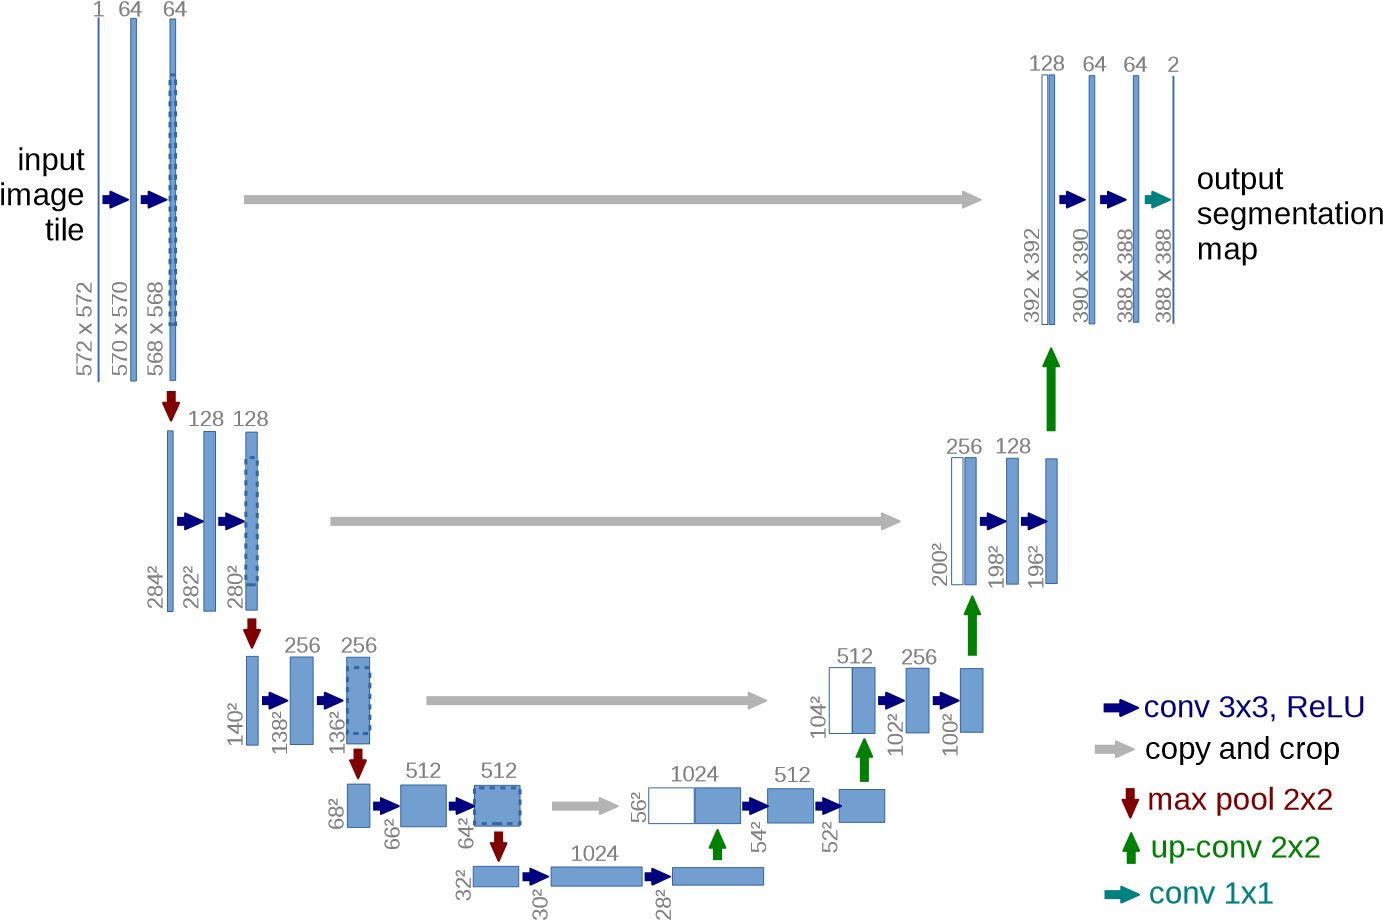
\includegraphics[width = 3.5in]{Unet_model}
    \caption{The network structure of Unet}
    \label{The network structure of Unet}
\end{figure}

The network structure of U-Net is shown in the figure 1.
It has a contracting path on the left side and an expansive path on the right side. \cite{DBLP:journals/corr/RonnebergerFB15}
The left side can be regarded as an encoder, and the right side can be regarded as a decoder.
The encoder has four sub-modules, each of which contains two convolutional layers.
After each sub-module, there is a down-sampling layer implemented by max pool.
The decoder contains four sub-modules, and the resolution is sequentially increased by upsampling until it is consistent with the resolution of the input image.
As the convolution uses the valid mode, the actual output is smaller than the input image.
The network also uses a skip connection to connect the upsampling result with the output of the sub-module with the same resolution in the encoder as the input of the next sub-module in the decoder.

\subsection{Unet++}
Medical image segmentation usually needs a higher accuracy than normal image segmentation because marginal segmentation errors in medical images can lead to strong uncertainties.
Besides, inaccurate segmentation may also lead to unsure changes in machine diagnosis.\cite{DBLP:journals/corr/abs-1807-10165}
The discovery of Unet++ helps recover more detailed information in medical images.


\begin{figure}[H]
    \centering
    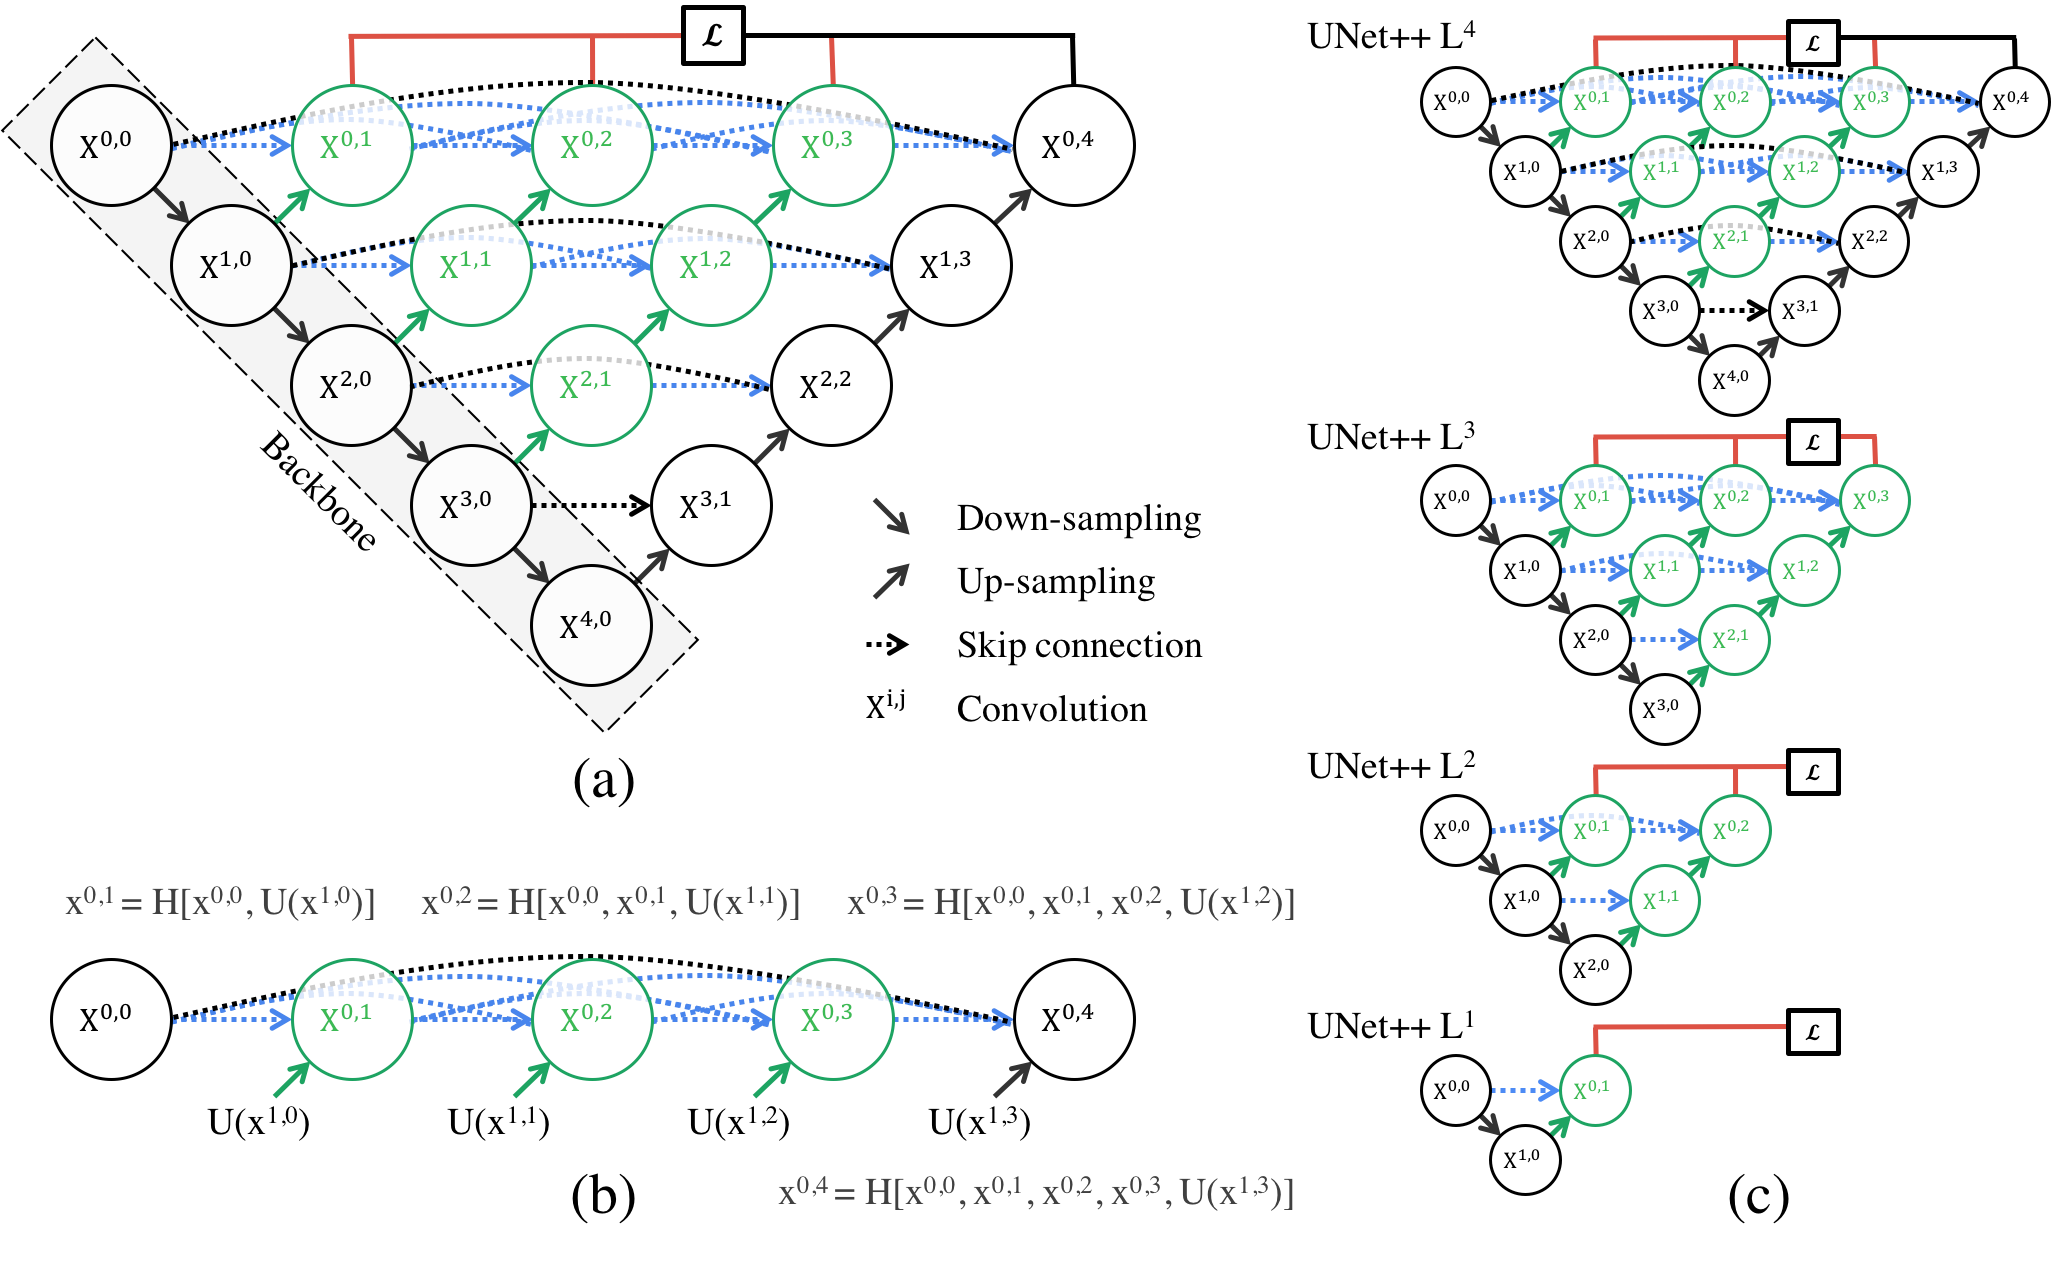
\includegraphics[width = 3.5in]{Unet++}
    \caption{The detail of Unet++}
    \label{The detail of Unet++}
\end{figure}


The figure2 shows some detail of the structure of the Unet++ network.
The subfigure (a) describes that UNet++ improves the encoder and the decoder by adding nested dense convolutional blocks.
So that UNet++ can bridge the semantic gap between the feature maps.
Lines in subfigure (b) illustrates the first skip pathway in Unet++.
Cause the Unet++ model can operate in the accurate mode in which all segmentation branches’ outputs are averaged, and the fast mode which only calculates the final result by selecting on a branch, deep supervision has been used in Unet++.
And the subfigure(c) shows the pruning procedure when the Unet++ model is trained in deep supervision.\cite{DBLP:journals/corr/abs-1807-10165,zhou2020unet}

\subsection{SegNet}
The figure shows the structure of SegNet.
The encoder network consists of 13 convolutional layers, which correspond to the first 13 convolutional layers in the VGG16 network \cite{simonyan2014very}, and every encoder network has its own corresponding decoder layer.\cite{DBLP:journals/corr/BadrinarayananK15}
The encoder network alternately uses convolutional layers and max pooling layers. On the contrary, the decoder uses de convolutional layers and upsampling layers.
And the softmax layer is used for pixel classification.

\begin{figure}[H]
    \centering
    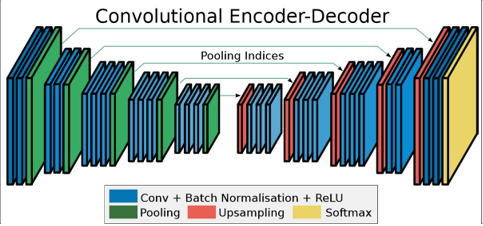
\includegraphics[width = 3.5in]{SegNet}
    \caption{The model of SegNet}
    \label{The model of SegNet}
\end{figure}

The max pooling layer can maintain translation invariance, so every pixel in the output feature map contains much of the input image's spatial information.
Because of translation invariance, the decoder network has strong robustness while loses information of boundary details, which is a great disadvantage.
So, a method that saves information of boundary details makes a great contribution to this network.
However, it is impossible to save all encoder feature maps (after downsampling).
Therefore, the model only stores the maximum pooling index, which is the location of the largest feature value in each pooling window used for each encoder feature map.

\subsection{Seg-Unet}
The figure shows the structure of Seg-Unet. The Seg-Unet model combines U-Net and Seg-Net, for Seg-Net has auto-encoder architecture, and Unet is fit for medical image segmentation.
This network is a newly developed one that not many researchers have studied.

\begin{figure}[H]
    \centering
    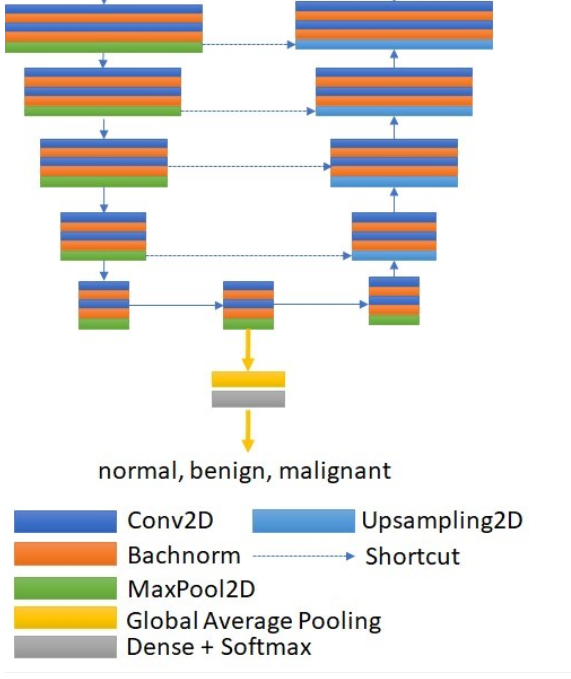
\includegraphics[width = 2.0in]{Seg-Unet}
    \caption{The model of Seg-Unet}
    \label{The model of Seg-Unet}
\end{figure}
\subsection{Res-Unet}
ResUNet combines the advantages of U-Net architecture and Residual neural network.
Generally the deeper the neural network, the better the performance of processing data, but usually there is no training algorithm to support it.
ResUNet balances the complexity and accuracy of network training to achieve better results.\cite{zhang2019zebrafish}
\subsubsection{U-Net}
In order to obtain a good segmentation effect, use low-level information while retaining high-level semantic information.
There are some good ways to solve this problem in U-net.
There are many ways to solve this problem in U-net, one of which is that it can expand the data.
In addition, U-net's own structure also helps to solve the training problem. U-net's own unique structure can not only supplement low-level language details to high-level semantic features, but also promote back propagation during training.\cite{zhang2018road}

\begin{figure}[H]
    \centering
    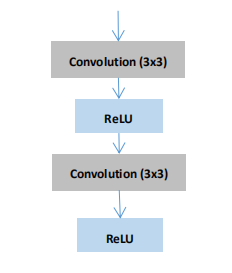
\includegraphics[width = 1.5in]{architecture of U-Net}
    \caption{The architecture of U-Net}
    \label{The architecture of U-Net}
\end{figure}
\subsubsection{Residual Network}
The idea of ResNet is to assume that we involve a network layer and there is an optimal network layer, so often the deep network we design has many network layers as redundant layers.
Then we hope that these redundant layers can complete the identity mapping to ensure that the input and output passing through the identity layer are exactly the same.
Which layer is the identity layer, this will be judged by yourself during network training.

\begin{figure}[H]
    \centering
    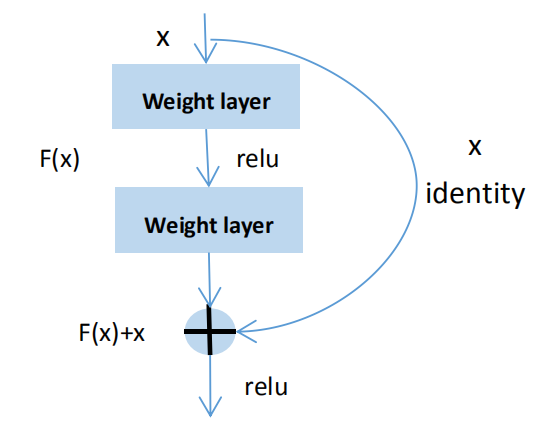
\includegraphics[width = 1.5in]{Residual Network}
    \caption{Residual Network: a building block}
    \label{Residual Network: a building block}
\end{figure}

It can be seen that X is the input of this layer of residual block, also called F(x) is the residual, x is the input value, F(X) is the output after the first layer of linear change and activation, the figure shows In the residual network, F(x) is added to the input value X of this layer before activation after the linear change of the second layer, and then output after activation. Add X before the activation of the output value of the second layer. This path is called a shortcut connection.
\subsubsection{ResUNet}
All pre-activated residual units are used to build deep ResUNet. Combining U-Net and Residual network will simplify the training of the network, build a neural network with fewer parameters, and achieve better results in semantic segmentation. The specific network structure is shown in the figure below.\cite{zhang2018road}

\begin{figure}[H]
    \centering
    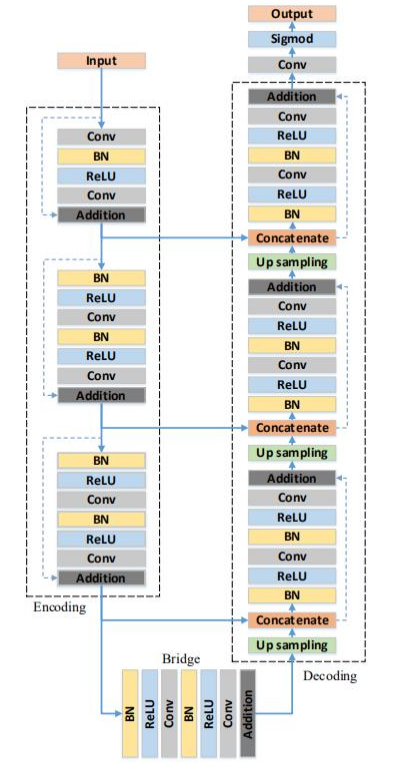
\includegraphics[width = 1.5in]{architecture of ResUNet}
    \caption{The architecture of ResUNet}
    \label{The architecture of ResUNet}
\end{figure}


\section{Experiment and Results}
In this section, the nuclei dataset used for the experiments, the evaluation measures, and lastly, the results are discussed in detail. It is important to note that the experiment was conducted under the Windows environment. The models were implemented in Tensorflow 1.15 and trained on the Nvidia GTX-1080Ti.

\subsection{Dataset}
The dataset is obtained from Kaggle 2018 Data Science Bowl\cite{kaggle_2018}, which consists of 735 nuclei images. The images were acquired under various conditions and vary in the cell type, magnification, and imaging modality. Each nuclei image is annotated with a series of masks marked by experts, and each image is represented by an associate ImageID. Files belonging to an image are contained in a folder with the ImageID, and within each folder, there are two subfolders:

\begin{itemize}
    \item[1.]“images” contains the image file
    \item[2.]“masks” contains the segmented masks of each nucleus.
\end{itemize}

In the pre-processing step, both training and testing data were down-sampled to keep the images light and manageable. The testing data's original sizes were recorded to up-sample the predicted masks and create correct run-length encodings later on. The pre-processing step is explained in a visual format on the simple example in Figure X. Among the dataset, 670 are used as training data, and 65 are chosen as testing data to measure the networks' performance.

\subsection{Evaluation Measures}
Generally speaking, semantic segmentation task performance can be measured based on two parameters: the Dice coefficient and the Jaccard coefficient. The Dice and the Jaccard coefficient is calculated by:
\begin{equation}
    Dice(A,B) = \frac{2\left \| A \cap B \right \|}{\left \| A \right \|+\left \| B \right \|}
\end{equation}
\begin{equation}
    Jaccard/IoU(A,B) = \frac{\left \| A \cap B \right \|}{\left \| A\cup B \right \|}
\end{equation}
In functions (1) and (2), A and B are two segmentation masks for a given class, $\left \| A \right \|$ is the norm of A, and $\cap$, $\cup$ are the intersection and union operators. Both the Dice and Jaccard indices are bounded between 0 (when there is no overlap) and 1 (when A and B match perfectly).

The Jaccard index is also known as Intersection over Union (IoU), and because of its intuitive and straightforward expression, it is widely used in computer vision applications. The IoU is used when calculating mean average precision. It is a number from 0 to 1 that specifies the overlap between the predicted and ground truth-bound boxes. An IoU of 0 means that there is no overlap between the boxes, and an IoU of 1 means that the union of the boxes is the same as their overlap, indicating that they are completely overlapping. IoU is an important accuracy measure to track when gathering human annotations. The Dice coefficient also called the overlap index, is the most used metric in validating medical volume segmentations. It has been widely used as a statistical validation metric to evaluate reproducibility.

Suprosanna et al.\cite{shit2020cldice} proposed a new metric called “clDice” that is able to evaluate tubular and linear structure segmentation based on intersecting skeletons with masks. Their finding is that training on clDice leads to segmentation with more accurate connectivity information, higher graph similarity, and often superior volumetric scores.
\begin{equation}
    Combined\;loss(\alpha=0.5) = (\alpha * Dice\;coefficent)+(\alpha * clDice\;coefficent)
\end{equation}

In the experiment, we adopt IoU as metrics and the combined loss as training loss. The combined loss consists of both Dice and clDice coefficient, the function is shown in (3) where we take half of the result from both the Dice and the clDice coefficient separately to form the final loss.

\subsection{Hyperparameter Setup}
Training of models is carried out using the weight optimizer Adam(Adaptive Moment Estimation). The learning step for all architectures is 0.0001. The batch size is set to 16, and the total epochs for all architectures are 60, while the validation split rate is 10\%. The early stopper is adopted with the patience of 15 steps to obtain the best-trained model. Meanwhile, the Reduce Learning Rate On Plateau function is used to avoid training struck on plateau. The function is set to monitor validation loss to adjust the learning step accordingly. The patience for the function is set to 5 steps, and the factor equals 10\%.

\subsection{Results}
Figure 8 represents the loss curve of Unet, Unet++, and ResUnet on the validation dataset. Notice that the epoch for each model is different as we adopt the early stopper at the training stage. The orange line denotes the loss on the training dataset, while the blue line represents the loss on the validation dataset. As shown in Figure 1, the three models' validation losses decrease as the number of epochs increases, and all of the three models are considered well fitted as there is no sign of overfitting or underfitting. However, the loss curve of SegNet and SegUnet is not that smooth as the three models mentioned above.
According to Figure 9, overfitting happened on the SegNet model as training loss is lower than validation loss, and the difference between training and validation losses seems to continue to expand with epoch. Besides, the validation loss curve is not smooth enough as there are many obvious changes on the curve. There is no sign of overfitting found on the SegUnet, but both training and validation losses are too high, which suggests that the model requires more epoch to be trained.

\begin{figure}[H]
    \subfigure[Unet]{
        \begin{minipage}[t]{0.33\linewidth}
            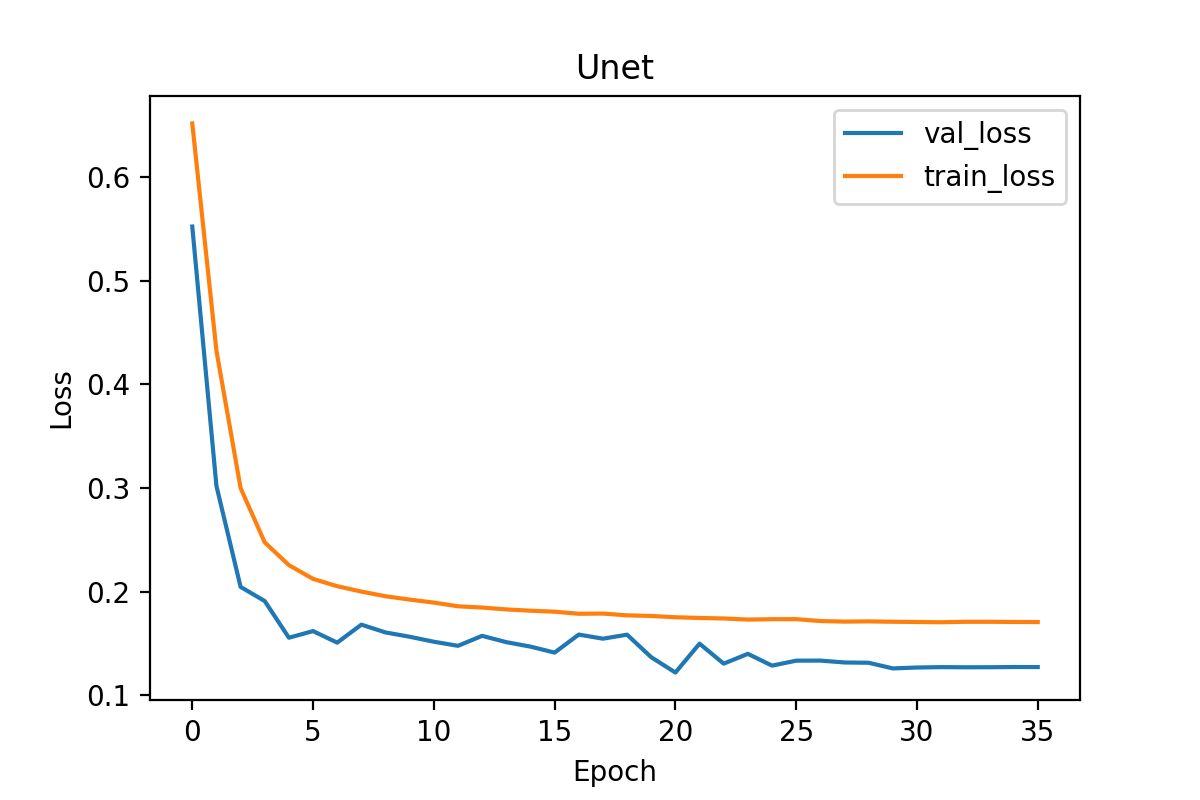
\includegraphics[width=4.3cm]{Unet_loss.png}
            %\caption{fig1}
        \end{minipage}%
    }%
    \subfigure[UnetPP]{
        \begin{minipage}[t]{0.33\linewidth}
            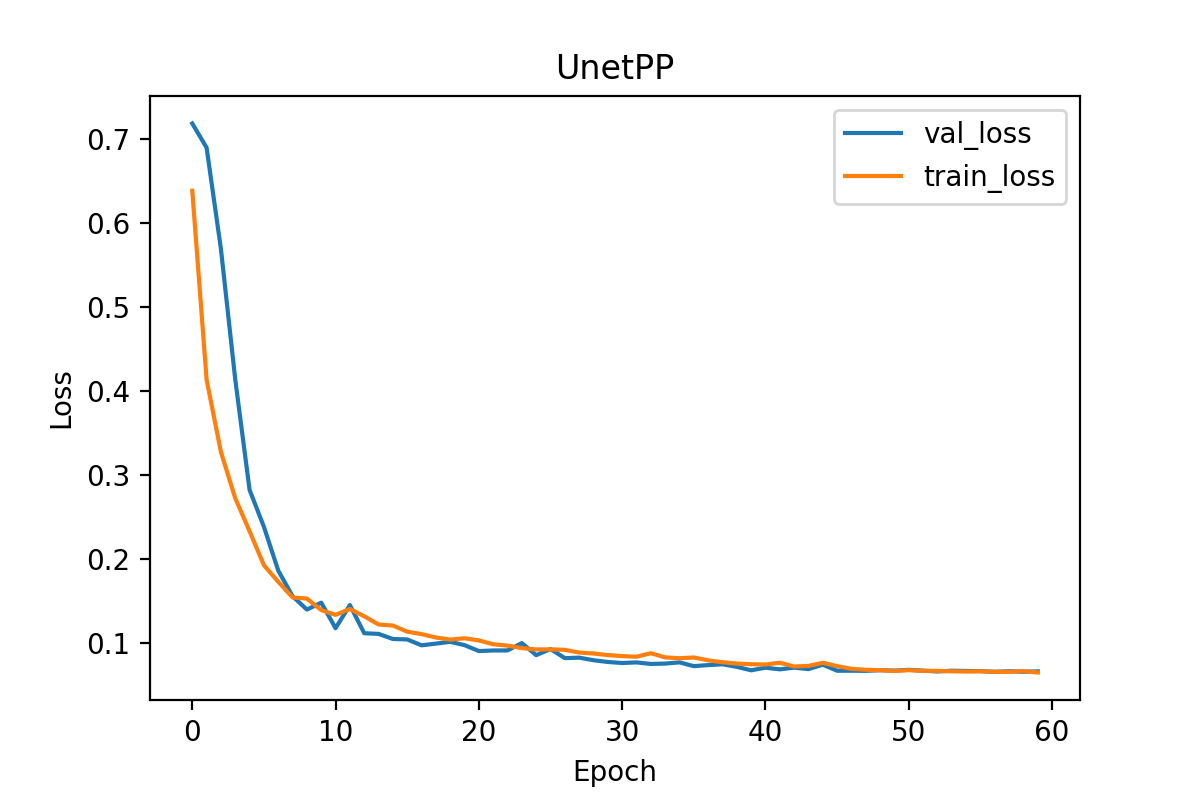
\includegraphics[width=4.3cm]{UnetPP_loss.png}
            %\caption{fig2}
        \end{minipage}%
    }%
    \subfigure[ResUNet]{
        \begin{minipage}[t]{0.33\linewidth}
            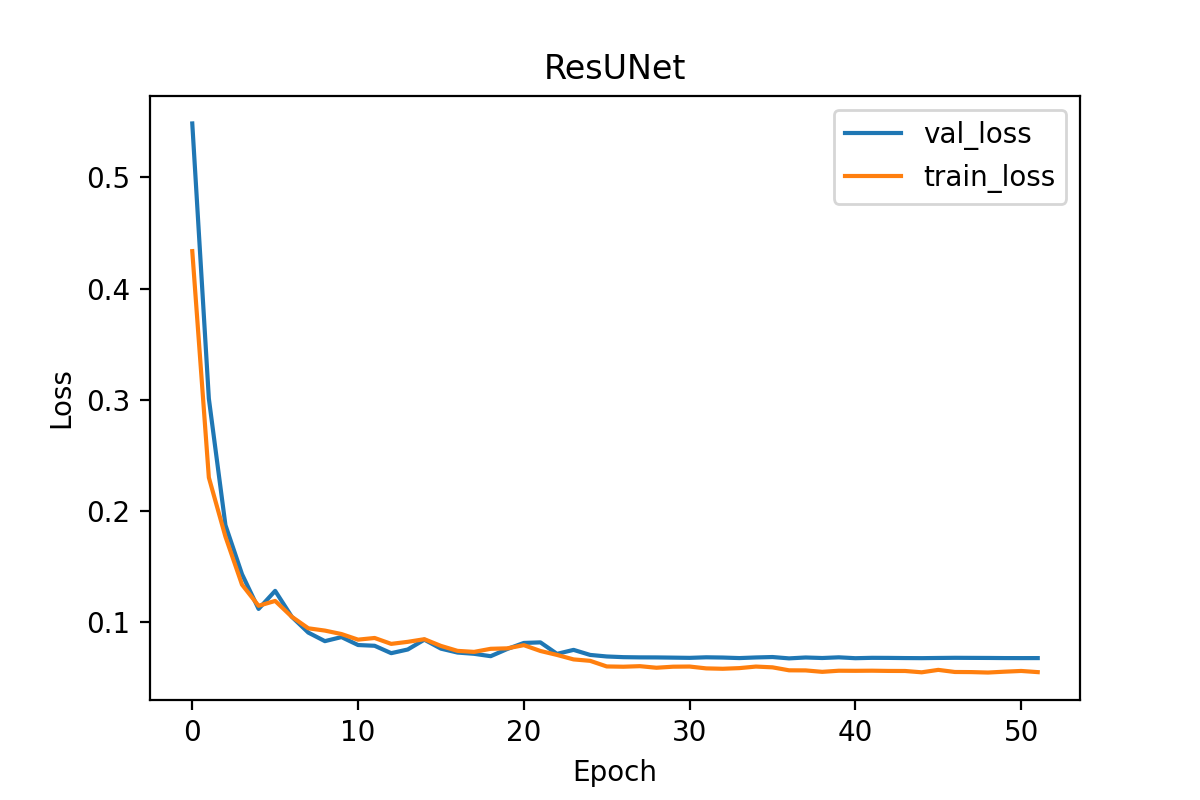
\includegraphics[width=4.3cm]{ResUNet_loss.png}
            %\caption{fig2}
        \end{minipage}
    }%
    \caption{Loss Curves of Unet, Unet++ and ResUNet}
\end{figure}

\begin{figure}[H]
    \subfigure[SegNet]{
        \centering
        \begin{minipage}[t]{0.5\linewidth}
            \centering
            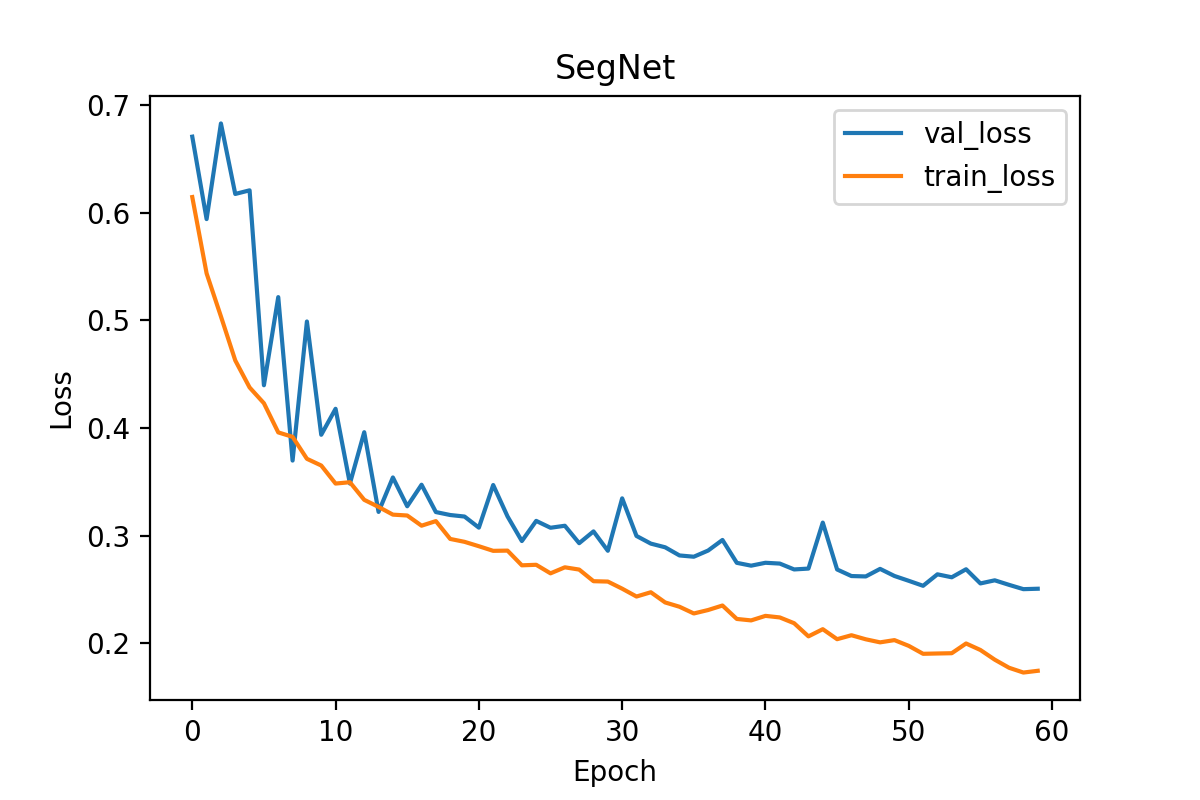
\includegraphics[width=4.3cm]{SegNet_loss.png}
        \end{minipage}
    }
    \subfigure[SegUNet]{
        \begin{minipage}[t]{0.5\linewidth}
            \centering
            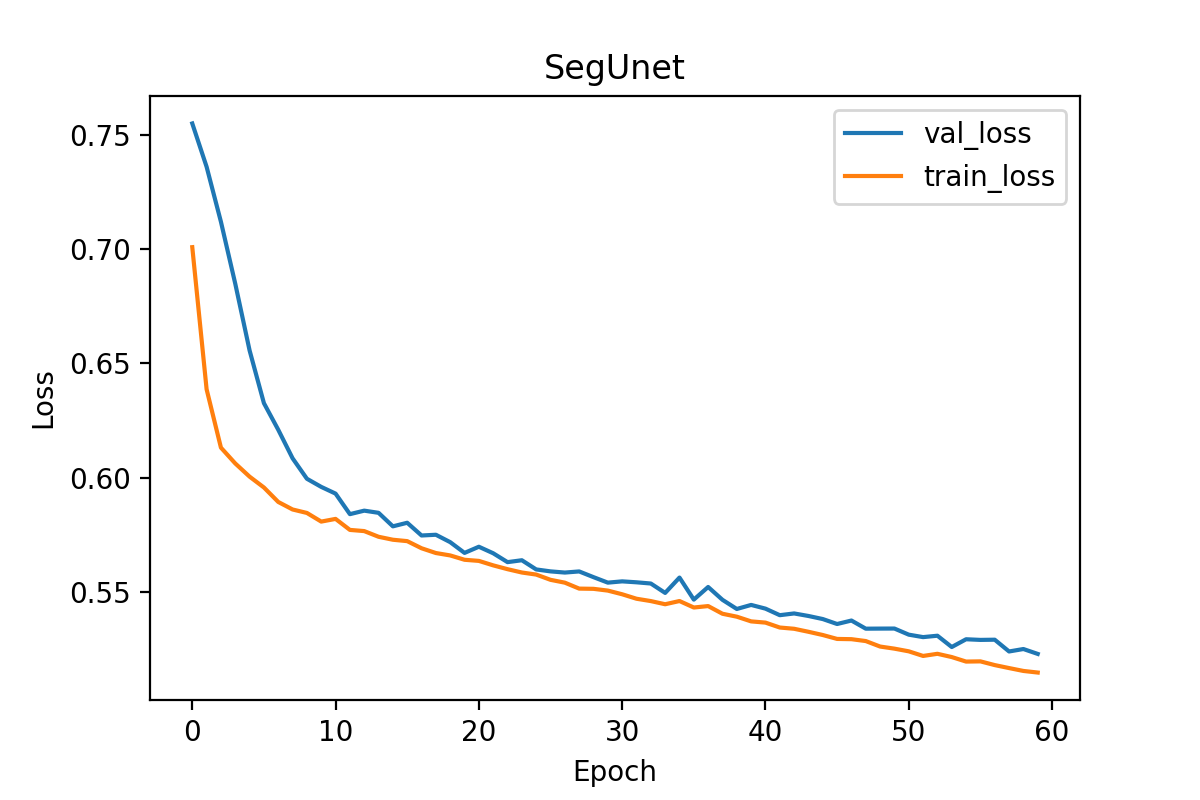
\includegraphics[width=4.3cm]{SegUnet_loss.png}
            \centering
        \end{minipage}
    }
    \caption{Loss Curves of SegNet and SegUNet}
\end{figure}

Figure 10 shows the segmentation results of different models on the testing dataset. The Unet, Unet++, and ResUnet show the correct segmentation for objects on the image border, while SegNet and SegUnet did not achieve a satisfactory result. For SegUnet, all the segmentation results are larger than the ground truth, indicating that the model is underfitting. While for SegNet, most of the segmentation results are in the wrong shape and connected with each other. One of the reasons that could cause this phenomenon is because SegNet does not have a U architecture to do down-sample and up-sample on the image like Unet.
\begin{figure}[H]
    \centering
    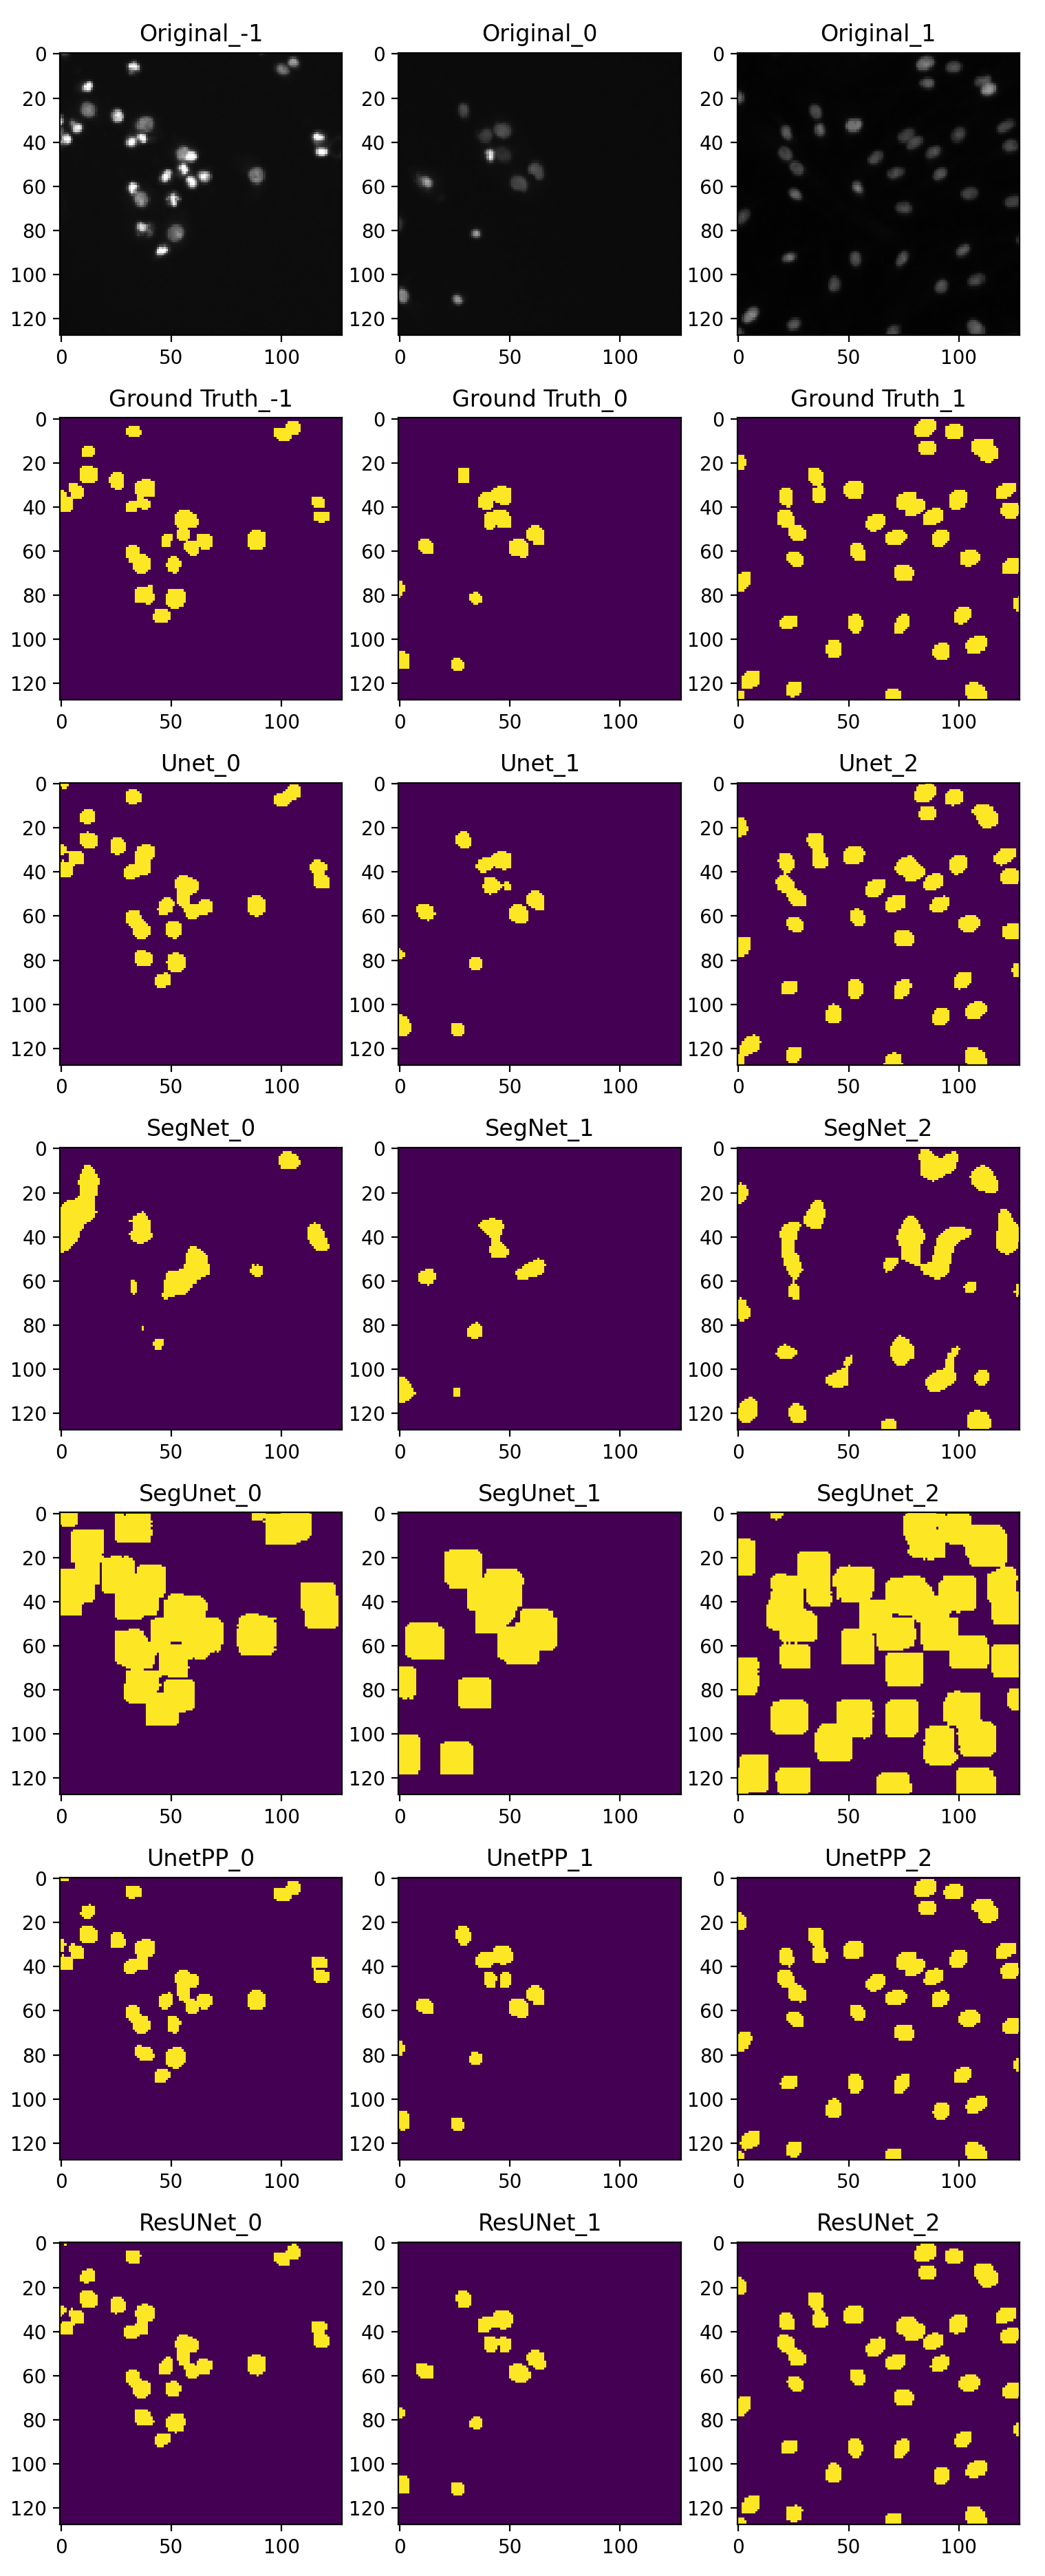
\includegraphics[width=9cm]{SegmentationResults.png}
    \caption{Original image, ground truth, and semantic segmentation performed with different models.}
    \label{2}
\end{figure}

Table 1 compares the performance of the five different models on the testing dataset. As we can see from the table, Unet++ obtains the highest dice score(0.929) among all the models, followed by ResUNet with a dice score of 0.9. The Unet has a relatively good score, while the performance of SegNet and SegUnet is not satisfactory, especially the SegUnet, which obtained the lowest score of 0.529.
\begin{table}[H]
    \begin{tabular}{@{}cccccc@{}}
        \toprule
        \textbf{}                     & \textbf{Unet}  & \textbf{Unet++} & \textbf{ResUnet} & \textbf{SegNet} & \textbf{SegUnet} \\ \midrule
        \textbf{Dice Coeffient(mean)} & \textbf{0.864} & \textbf{0.929}  & \textbf{0.92}    & \textbf{0.734}  & \textbf{0.529}   \\ \bottomrule
    \end{tabular}
    \caption{Comparison of the neural network accuracy for the testing dataset}
\end{table}

\section{Conclusion}
In the current study, we compared five different semantic segmentation models that include Unet, Unet++, ResUnet, SegNet, and SegUnet. The comparison was performed on the Kaggle nuclei image dataset. The result indicates that Unet++ has the best quality of segmentation in comparison with other networks. Further studies are connected with changing encoder net of different models. Instead of using common encoders, it would be better to use ResNet and Inseption for feature extraction.

\bibliography{bibfile}
\end{document}